\documentclass[11pt]{article}

\usepackage[margin=1in]{geometry}
\usepackage[T1]{fontenc}
\usepackage[utf8]{inputenc}
\usepackage{booktabs}
\usepackage{tabularx}
\usepackage{array}
\usepackage{longtable}
\usepackage{graphicx}
\usepackage{xcolor}
\usepackage{hyperref}
\usepackage{enumitem}
\usepackage{listings}
\usepackage{fancyhdr}

\hypersetup{
  colorlinks=true,
  linkcolor=blue!60!black,
  urlcolor=blue!60!black
}

\definecolor{codebg}{RGB}{247,247,247}
\definecolor{codeframe}{RGB}{220,220,220}

\lstdefinestyle{repo}{
  basicstyle=\ttfamily\small,
  backgroundcolor=\color{codebg},
  frame=single,
  rulecolor=\color{codeframe},
  columns=fullflexible,
  keepspaces=true,
  showstringspaces=false,
  breaklines=true
}

\newcolumntype{Y}{>{\raggedright\arraybackslash}X}

\pagestyle{fancy}
\fancyhf{}
\lhead{BNN\_FCC Submission Report}
\rhead{\thepage}

\title{\textbf{BNN\_FCC Contest Submission Report}}
\author{
  Khan Thamid Hasan \\
  UFID: 17308681 \\
  \texttt{khanthamidhasan@ufl.edu}
}
\date{April 17, 2026}

\begin{document}

\maketitle
\thispagestyle{empty}

\begin{center}
\begin{tabular}{ll}
Repository root: & \texttt{bnn\_fcc\_contest} \\
Top-level DUT: & \texttt{rtl/bnn\_fcc.sv} \\
Timing target: & \texttt{XCU250-FIGD2104-2L-E} \\
Canonical candidate: & \texttt{PARALLEL\_INPUTS = 8,\ PARALLEL\_NEURONS = \{8,8,1\}} \\
\end{tabular}
\end{center}

\section*{Executive Summary}

\begin{tabularx}{\textwidth}{@{}lY@{}}
\toprule
Item & Result \\
\midrule
Targeted use case & High-frequency, BRAM-backed implementation with conservative output-layer parallelism \\
Required topology & MNIST SFC: \texttt{784 -> 256 -> 256 -> 10} \\
Canonical submission parameters & \texttt{PARALLEL\_INPUTS = 8}, \texttt{PARALLEL\_NEURONS = \{8,8,1\}} \\
Openflex timing flow & PASS \\
Measured $f_{max}$ & \textbf{400.48 MHz} \\
LUTs & \textbf{3066} \\
FFs & \textbf{1818} \\
BRAM & \textbf{12.5} \\
DSP & \textbf{0} \\
Additional coverage testbench & PASS, average covergroup score \textbf{96.1\%} \\
Performance-oriented simulation run & PASS, with reported results from \texttt{sim/perf\_out.txt} listed in Section~\ref{sec:perf} \\
\bottomrule
\end{tabularx}

\paragraph{Submission note.}
During final repo cleanup, the default \texttt{PARALLEL\_NEURONS} setting in \texttt{verification/bnn\_fcc\_tb.sv} was synchronized with the DUT and timing wrapper so that the design being documented, verified, and timed is the same candidate. If you regenerate logs after that synchronization, update the small numerical tables in Sections~\ref{sec:verification-results} and~\ref{sec:perf} before producing the final PDF.

\section{Design Objective and Tradeoff}

This submission targets a believable high-frequency operating point on the provided UltraScale+ target rather than maximum raw output-layer spatial parallelism. The main architectural tradeoff is to keep the hidden layers moderately parallel while serializing the small output layer:

\begin{itemize}[leftmargin=1.5em]
\item \texttt{PARALLEL\_INPUTS = 8}
\item Hidden-layer parallelism: \texttt{PARALLEL\_NEURONS[0] = 8}, \texttt{PARALLEL\_NEURONS[1] = 8}
\item Output-layer parallelism: \texttt{PARALLEL\_NEURONS[2] = 1}
\end{itemize}

The intent is to reduce routed timing pressure on the BRAM $\rightarrow$ XNOR $\rightarrow$ popcount $\rightarrow$ accumulate path while keeping memory organization simple and timing-friendly. This approach favors a stronger timing result and a smaller, cleaner hardware footprint at the cost of some end-to-end throughput relative to a more spatially aggressive output layer.

\section{Repository Structure}

\begin{tabularx}{\textwidth}{@{}lY@{}}
\toprule
Path & Purpose \\
\midrule
\texttt{rtl/} & Top-level DUT and interface specification \\
\texttt{verification/} & Required functional testbench plus additional coverage-oriented testbench \\
\texttt{openflex/} & Openflex YAML flows, timing wrapper, helper parser patch, and flow notes \\
\texttt{python/} & Model data and reference test vectors used by the testbench infrastructure \\
\texttt{doc/} & Background slides and supporting material \\
\texttt{report.tex} & Canonical source for the submission report \\
\bottomrule
\end{tabularx}

\section{How to Run the Repository}

\subsection{Prerequisites}

\begin{itemize}[leftmargin=1.5em]
\item Siemens Questa/ModelSim for simulation
\item Xilinx Vivado for synthesis, place, and route
\item Python virtual environment containing \texttt{openflex}
\item Linux shell environment for the contest flows
\end{itemize}

\subsection{Build a local simulator work library}

From the repository root:

\begin{lstlisting}[style=repo,language=bash]
mkdir -p sim
cd sim
vlib work

vlog -sv ../rtl/bnn_fcc.sv \
         ../verification/axi4_stream_if.sv \
         ../verification/bnn_fcc_tb_pkg.sv \
         ../verification/bnn_fcc_tb.sv \
         ../verification/bnn_fcc_coverage_tb.sv \
         ../openflex/rtl/bnn_fcc_timing.sv
\end{lstlisting}

\subsection{Required functional simulation}

This is the direct simulation of the provided top-level testbench:

\begin{lstlisting}[style=repo,language=bash]
vsim -c work.bnn_fcc_tb -do "run -all; quit -f" | tee tb_out.txt
grep -E "SUCCESS:|FAILED:|Avg latency|Avg throughput" tb_out.txt
\end{lstlisting}

\subsection{Performance-oriented simulation}
\label{sec:perf-cmd}

To measure performance without external throttling, use the measured timing result as the clock period and disable randomized source/sink stalls:

\begin{lstlisting}[style=repo,language=bash]
vsim -c work.bnn_fcc_tb \
  -gCLK_PERIOD=2.497ns \
  -gTOGGLE_DATA_OUT_READY=0 \
  -gCONFIG_VALID_PROBABILITY=1.0 \
  -gDATA_IN_VALID_PROBABILITY=1.0 \
  -do "run -all; quit -f" | tee perf_out.txt

grep -E "SUCCESS:|Avg latency|Avg throughput" perf_out.txt
\end{lstlisting}

\subsection{Coverage-oriented simulation}

The repository includes an additional self-checking coverage testbench:

\begin{lstlisting}[style=repo,language=bash]
vsim -c work.bnn_fcc_coverage_tb -do "run -all; quit -f" | tee coverage_tb_out.txt
tail -n 40 coverage_tb_out.txt
\end{lstlisting}

\subsection{Openflex verification and timing flows}

From the repository root:

\begin{lstlisting}[style=repo,language=bash]
cd openflex
source ~/envs/openflex/bin/activate
\end{lstlisting}

If openflex crashes while parsing a completed Vivado run because Vivado reports fractional utilization values such as \texttt{12.5} BRAMs, patch the installed parser:

\begin{lstlisting}[style=repo,language=bash]
python patch_openflex_parser.py --check
python patch_openflex_parser.py
\end{lstlisting}

Then run the canonical contest flows:

\begin{lstlisting}[style=repo,language=bash]
openflex bnn_fcc_verify.yml | tee verify_out.txt
openflex bnn_fcc_coverage.yml | tee coverage_out.txt
openflex bnn_fcc_timing.yml -c bnn_fcc.csv | tee timing_out.txt
\end{lstlisting}

Useful summaries:

\begin{lstlisting}[style=repo,language=bash]
grep -E "SUCCESS:|FAILED:|FAILURE:" verify_out.txt
grep -E "WNS|Post Physical Optimization Timing Summary|8-7052|8-7030|8-6904" timing_out.txt
cat bnn_fcc.csv
\end{lstlisting}

\subsection{Build the submission PDF}

From the repository root:

\begin{lstlisting}[style=repo,language=bash]
latexmk -pdf report.tex
\end{lstlisting}

If \texttt{latexmk} is unavailable:

\begin{lstlisting}[style=repo,language=bash]
pdflatex report.tex
pdflatex report.tex
\end{lstlisting}

\section{Architecture Summary}

\subsection{Top-level functionality}

The DUT implements a parameterized fully connected binary neural network classifier with three AXI4-Stream interfaces:

\begin{itemize}[leftmargin=1.5em]
\item Configuration input for weights and thresholds
\item Image input stream for 8-bit pixels
\item Output stream for the predicted class index
\end{itemize}

The reference contest topology is the small fully connected FINN-style network:

\begin{center}
\texttt{784 inputs -> 256 hidden -> 256 hidden -> 10 outputs}
\end{center}

\subsection{Key implementation choices}

\begin{itemize}[leftmargin=1.5em]
\item The configuration stream is parsed internally from the provided message headers rather than assuming a single fixed message order.
\item Image pixels are binarized against \texttt{8'd128} to match the provided verification model.
\item Weights are stored in packed words with width \texttt{PARALLEL\_INPUTS = 8}, enabling BRAM-backed storage that matches the datapath width.
\item Threshold memories for the hidden layers are inferred as LUTRAM, which Vivado reports as the efficient choice for the threshold array sizes in this design.
\item Inference proceeds layer by layer, with hidden layers producing binarized activations and the output layer performing argmax over population counts.
\item Output backpressure is honored by holding a valid result until \texttt{data\_out\_ready} is asserted.
\end{itemize}

\subsection{Timing-oriented refinements}

The latest submission candidate includes several low-risk timing improvements:

\begin{itemize}[leftmargin=1.5em]
\item The popcount across the 8-bit XNOR word is implemented as a fixed balanced tree rather than a generic loop-based reduction.
\item The output layer is serialized by choosing \texttt{PARALLEL\_NEURONS[2] = 1}, which reduces pressure on the routed critical path.
\item The BRAM weight bank logic was restructured to present a cleaner read/write organization to synthesis.
\item The hidden-layer parallelism remains matched to \texttt{PARALLEL\_INPUTS} to preserve straightforward packing and inter-layer buffering.
\end{itemize}

\section{Verification Strategy}

\subsection{Required contest testbench}

The required functional verification infrastructure is the provided \texttt{verification/bnn\_fcc\_tb.sv}. It checks:

\begin{itemize}[leftmargin=1.5em]
\item Correct parsing and loading of the trained model
\item Correct MNIST classification outputs
\item Robustness to randomized \texttt{config\_valid} gaps
\item Robustness to randomized \texttt{data\_in\_valid} gaps
\item Robustness to randomized \texttt{data\_out\_ready} backpressure
\item Reported latency and throughput statistics
\end{itemize}

\subsection{Additional coverage-oriented testbench}

The repository also includes \texttt{verification/bnn\_fcc\_coverage\_tb.sv}, which was added specifically to improve verification quality beyond the basic contest pass/fail flow. This testbench stresses:

\begin{itemize}[leftmargin=1.5em]
\item Reordered configuration messages
\item Partial \texttt{TKEEP} on both configuration and image traffic
\item Reset during configuration and reset during image streaming
\item Continuous, random, and bursty valid / ready behavior
\item Repeated outputs versus varying outputs
\item Coverage of all output classes in a self-checking randomized scenario
\end{itemize}

The coverage testbench prints both a success banner and a per-covergroup summary, which makes it easy for an evaluator to inspect coverage quality without digging into simulator databases.

\section{Results}

\subsection{Timing and resource utilization}

The measured timing and area results from \texttt{openflex/bnn\_fcc.csv} are summarized below.

\begin{center}
\begin{tabular}{lr}
\toprule
Metric & Value \\
\midrule
$f_{max}$ & 400.48057669203047 MHz \\
LUT & 3066 \\
LUT as logic & 2298 \\
LUT as memory & 768 \\
FF / registers & 1818 \\
BRAM & 12.5 \\
DSP & 0 \\
\bottomrule
\end{tabular}
\end{center}

Vivado also reports the expected memory implementation split for this architecture:

\begin{itemize}[leftmargin=1.5em]
\item Weight banks inferred into BRAM
\item Threshold memories inferred into LUTRAM because BRAM would be inefficient for the small threshold arrays
\item Timing warnings indicating that optional BRAM output registers were not merged, which is consistent with the remaining critical path pressure reported during implementation
\end{itemize}

\subsection{Verification and coverage results}
\label{sec:verification-results}

The additional coverage-oriented run reported the following summary:

\begin{center}
\begin{tabularx}{\textwidth}{@{}lY@{}}
\toprule
Covergroup / check & Result \\
\midrule
\texttt{config\_msg\_cov} & 95.8\% \\
\texttt{keep\_cov} & 85.4\% \\
\texttt{valid\_mode\_cov} & 100.0\% \\
\texttt{ready\_mode\_cov} & 100.0\% \\
\texttt{reset\_cov} & 100.0\% \\
\texttt{output\_cov} & 100.0\% \\
\texttt{output\_seq\_cov} & 100.0\% \\
\texttt{threshold\_cov} & 94.4\% \\
\texttt{weight\_cov} & 88.9\% \\
Average covergroup score & \textbf{96.1\%} \\
Pass / fail banner & \texttt{SUCCESS: bnn\_fcc\_coverage\_tb completed with 16 passing checks.} \\
\bottomrule
\end{tabularx}
\end{center}

\subsection{Performance-oriented run}
\label{sec:perf}

The latest supplied direct performance run from \texttt{sim/perf\_out.txt} reported:

\begin{center}
\begin{tabularx}{\textwidth}{@{}lY@{}}
\toprule
Metric & Value \\
\midrule
Pass / fail banner & \texttt{SUCCESS: all 50 tests completed successfully.} \\
Average latency & 89694.8 cycles / image \\
Average latency (time) & 223968.0 ns / image \\
Average throughput & 4464.5 outputs / sec \\
Average cycles / output & 89704.3 \\
\bottomrule
\end{tabularx}
\end{center}

\paragraph{Important cleanup note.}
Because the required testbench defaults were synchronized during final repository cleanup, this performance table should be refreshed after rerunning the command in Section~\ref{sec:perf-cmd} if you want every reported number in the PDF to correspond exactly to the final repository state.

\subsection{Representative console snapshot}

Figure~\ref{fig:console-snapshot} shows a representative terminal capture from the final verification workflow. The image includes the passing coverage summary and the performance-oriented testbench statistics that were used when preparing this submission package.

\begin{figure}[htbp]
\centering
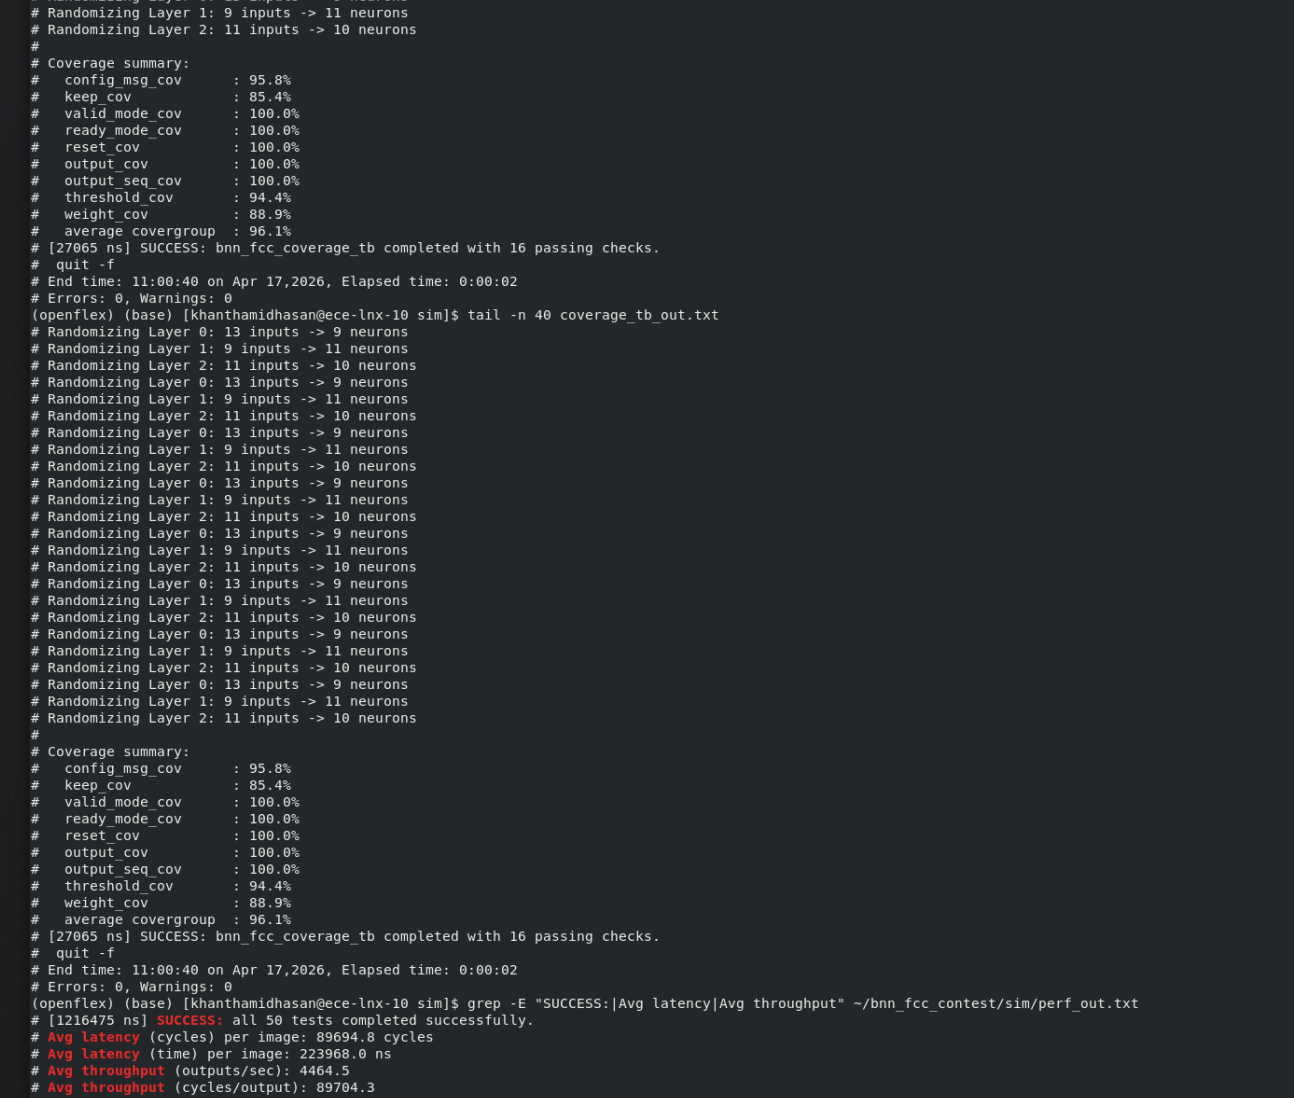
\includegraphics[width=0.94\textwidth,height=0.78\textheight,keepaspectratio]{images/final_console_snapshot.png}
\caption{Representative terminal snapshot showing the final coverage summary and performance-oriented simulation results.}
\label{fig:console-snapshot}
\end{figure}

\section{Why This Is a Reasonable Contest Candidate}

This submission is credible for the contest because it makes a coherent and defensible tradeoff:

\begin{itemize}[leftmargin=1.5em]
\item It does not rely on unrealistic outlier timing claims. The measured $f_{max}$ is in a believable range for a BRAM-backed UltraScale+ design.
\item It keeps resource use small: only 3066 LUTs, 1818 FFs, 12.5 BRAMs, and 0 DSPs.
\item It includes extra verification infrastructure rather than only the minimum required contest testbench.
\item The repo contains the exact files needed to rerun functional verification, coverage, and timing from the command line.
\end{itemize}

\section{Submission Checklist}

Before turning in the repository, the following should be true:

\begin{enumerate}[leftmargin=1.5em]
\item \texttt{verification/bnn\_fcc\_tb.sv}, \texttt{verification/bnn\_fcc\_coverage\_tb.sv}, \texttt{rtl/bnn\_fcc.sv}, and \texttt{openflex/rtl/bnn\_fcc\_timing.sv} all use the same canonical submission parameters.
\item The required functional simulation passes with no failing tests.
\item The additional coverage-oriented simulation passes and prints the coverage summary.
\item \texttt{openflex bnn\_fcc\_verify.yml} passes.
\item \texttt{openflex bnn\_fcc\_timing.yml -c bnn\_fcc.csv} completes and reports the expected timing / area values.
\item \texttt{report.pdf} is rebuilt from this \texttt{report.tex} source after the final verification and timing reruns.
\end{enumerate}

\section*{Appendix: Exact Commands}

\begin{lstlisting}[style=repo,language=bash]
# compile
mkdir -p sim
cd sim
vlib work
vlog -sv ../rtl/bnn_fcc.sv \
         ../verification/axi4_stream_if.sv \
         ../verification/bnn_fcc_tb_pkg.sv \
         ../verification/bnn_fcc_tb.sv \
         ../verification/bnn_fcc_coverage_tb.sv \
         ../openflex/rtl/bnn_fcc_timing.sv

# required simulation
vsim -c work.bnn_fcc_tb -do "run -all; quit -f" | tee tb_out.txt

# performance simulation
vsim -c work.bnn_fcc_tb \
  -gCLK_PERIOD=2.497ns \
  -gTOGGLE_DATA_OUT_READY=0 \
  -gCONFIG_VALID_PROBABILITY=1.0 \
  -gDATA_IN_VALID_PROBABILITY=1.0 \
  -do "run -all; quit -f" | tee perf_out.txt

# coverage simulation
vsim -c work.bnn_fcc_coverage_tb -do "run -all; quit -f" | tee coverage_tb_out.txt

# openflex
cd ../openflex
source ~/envs/openflex/bin/activate
python patch_openflex_parser.py --check
python patch_openflex_parser.py
openflex bnn_fcc_verify.yml | tee verify_out.txt
openflex bnn_fcc_coverage.yml | tee coverage_out.txt
openflex bnn_fcc_timing.yml -c bnn_fcc.csv | tee timing_out.txt

# build report
cd ..
latexmk -pdf report.tex
\end{lstlisting}

\end{document}
